\section{How can we improve it with MPI ?}
In this section, we'll talk about hashtables (of my personnal design, because it allowed to add some optimization in the hashtables itselves).

\subsection{Occurences counting}
The counting of the number of occurences for each character is a part where parallisation can be very interesting.\\
The current design of my MPI version of this part is the following :\\
\begin{itemize}
	\item Each process create a personnal hashtable and a final hashtable
	\item Each process has a part of the file to read in order to count the occurences of each character, which will be stored in the personnal hashtable
	\item When its done, the secondaries processes will send to the primary process several informations
	\begin{itemize}
		\item Number of entries in its personnal table
		\item For each entry, the character associated and its number of occurences
	\end{itemize}
	\item The primary process will then one secondary process at the time, gather those informations, and add it in its final table.
	\item When it's done, it will also add its personnal table information in its final table.\\
	Now the primary process has a final table which all the information about the characters in the file.
	\item And finally, it will broadcast its final table to each secondary process
\end{itemize}
Here is a diagram of the communication when we're using 4 process :
\begin{figure}[H]
\centering
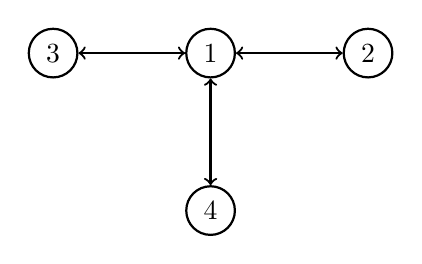
\begin{tikzpicture}[node distance={20mm}, thick, main/.style = {draw, circle}] 
\node[main] (1) {$1$}; 
\node[main] (2) [right of=1] {$2$}; 
\node[main] (3) [left of=1] {$3$};
\node[main] (4) [below of=1] {$4$};
\draw[<->] (1) -- (2);
\draw[<->] (1) -- (4);
\draw[<->] (1) -- (3);
\end{tikzpicture} 
\caption{Communication diagram of this part, everything goes through the primary, node "1"}
\label{fig:my_label}
\end{figure}

\subsection{Compression}
The compression part proceed in a different way. A problem of this part is that we have to write the compressed data in the right order, so each process has to wait for the previous to end its writing in order for him to start.\\
And, we could think that there is no reason to parallelize this part, but there is one job that is done by each process that can be done by all of them during the same time.\\
Each of them, before writing in the output file will produce a buffer containing the compressed data.\\
This job include walking through the hashtable several times and some computation. This isn't a truly expensive job so the gain from this parallelization isn't as big as expected but it is still an interesting algorithm.\\
\\
Due to the problem that I spoke earlier, each process will have to write sequentially and in order.\\
Also, our process are writing sequence of bits, so when it is done writing, it might not have wrote everything is supposed to.\\
For example, if the process \textit{i} was about to write a new byte containing the sequence "0010" but has nothing else to put to complete the byte, it will have to transmit what it was going to write ("0010") to the next process \textbf{i+1} in order for it to complete the byte with bits that it is supposed to write.\\
This mechanism create an one-to-one communication between each process \textbf{i} to a process \textbf{i+1}.\\
Here is a diagram of the communication when we're using 4 process :
\begin{figure}[H]
\centering
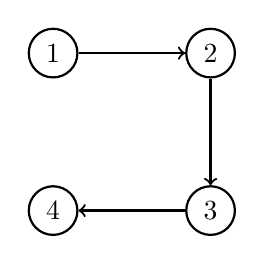
\begin{tikzpicture}[node distance={20mm}, thick, main/.style = {draw, circle}] 
\node[main] (1) {$1$}; 
\node[main] (2) [right of=1] {$2$}; 
\node[main] (3) [below of=2] {$3$};
\node[main] (4) [below of=1] {$4$};
\draw[->] (1) -- (2);
\draw[->] (2) -- (3);
\draw[->] (3) -- (4);
%\draw[->] (4) -- (1);
\end{tikzpicture} 
\caption{Communication diagram of this part, everything goes through the primary, node "1"}
\label{fig:my_label}
\end{figure}

\subsection{Decompression, what's the problem ?}
The decompression have some of the issues of the compression. We can't have several processes writing in the same output file in the same time.\\
\\
We could try to parallelize the decompression main part, which is reading from the input file and convert sequence of bits into characters.\\
But one of the issue with this is that, what if a process \textbf{i} has reach the end of the input file, but hasn't a complete sequence of bits (one corresponding to one character). This means that the remaining part of the sequence will be in the part of the input file of the next process \textbf{i+1}.\\
So in order for the process \textbf{i} to complete its job, it would have to communicate with the process \textbf{i+1} in order to have the missing bits. And the process \textbf{i+1} will have to do the same with the process \textbf{i+2}, etc...\\
\\
And in order for that to work, a process \textbf{i+1} would have to transmit the missing bits to the previous process \textbf{i}. But how can it determine how much bits are missing ?\\
For now, I don't have a solution to this question. If I found one, I would be able to try to parallelize the decompression, but I'm not sure that it would have a huge impact on the performance.

\section{Results}
It is hard for me to study the performance of my algorithm for 2 reasons :
\begin{itemize}
	\item It seems like when the file get too big, the program will crash due to a memory allocation too big to be handled.
	\item Also, I wasn't able to use Grid'5000, launching my MPI version on Grid'5000 crash for an unknown reason.
\end{itemize}
But I was still able to have a glance to the gains offered by my version.\\
\begin{figure}[H]
    \centering
    \includegraphics[scale=0.8]{img/chart.png}
    \caption{Chart produced using the simple "time" unix tool}
    \label{fig:my_label}
\end{figure}
Each segment correspond to a different type of execution :
\begin{itemize}
	\item huffman.std : Execution done by my standard version of the Huffman Algorithm
	\item huffman.mpi.\textbf{n} : Execution done by my MPI version of the Huffman Algorithm, using \textbf{n} process
\end{itemize}

\section{Conclusion}
It is indeed possible to upgrade a Huffman algorithm using parallelization but the upgrade has to be study well before being implemented, because this algorithm is fundamantally executed sequentially.\\
In my study I have only done upgrades on the compression part, and for now, I don't have any idea for an upgrade of the decompression part.